\chapter{Narukom}
\label{Narukom}

\section{Name}
Before we dive into the technical details about narukom,  we spare a little time in order to explain why we gave the name Narukom to our framework. In the beginning, the name was Kouretes System of Communication ( KouSoCom ), but after watching approximately 300 episodes of the popular Japanese cartoon (a.k.a anime) Naruto in less than ten days, so we decided to include Naruto in the title. As a result KouSoCom became Narukom from the combination of the words Naruto, Kouretes and Communication.

\section{The Concept}
After the adoption of the Nao platform , our team did not have a framework to share information between the robots. The majority of the messages was quick hacks developed by individuals which made the code maintenance infeasible, thus  the need for a well defined, easy to use framework emerged. The proposed communication framework, Narukom, tries to address the communication needs of robotic teams by providing an efficient, flexible, and simple way of exchanging messages between robots, without imposing restrictions on the type of the data transferred over the network.

\section{Architecture}

\subsection{Overview}

Narukom's main idea is a topic-based publish/subscribe system for exchanging messages locally  or over the network \footnote[1]{ Apart from  robot-to-robot communication, Narukom is used also for robot-to-computer communication , so we refer to both systems ( robots and computers ) as network nodes or shortly nodes.}. On each node there is only one instance of  an intermediate broker (Message Queue), that temporarily stores published messages and delivers copies 
to the interested subscribers. The Message Queue holds a hierarchical topic tree, which is used for subscribing to messages on a particular topic ({\tt
on\_topic}) or on a topic and its ancestors ({\tt above\_topic}) or on a topic and its descendants ({\tt below\_topic}).

\subsection{Narukom in Robocup}

A robotic agent is composed of modules that implement different concrete functionalities. The idea that modules produce data for other modules and use data from other modules comes quite natural, as , for example the behavior module depends on data from localization module and the object recognition module uses  color-segmented image from the image segmentation module. In our team's architecture, modules that operate on the same data are grouped in a thread. Threads are perceived as publishers or subscribers (or both), which could publish data on certain topics or receive  data by subscribing to certain topics. In order to simplify the way threads or modules share such data, Narukom introduces a distributed Blackboard design, whereby modules from different threads on the same or even different network nodes access transparently the desired data. 

\subsection{Blackboard}

A Blackboard module  in the context of the publish/subscribe paradigm is simply a subscriber, which  serves other module requests for data, stored internally and published by modules or threads on the same or remote node. There could be either one blackboard for all the modules/threads of a robot or multiple blackboards, one for each thread running on the robot. Our team adopted the later design , because of the synchronization problems occurring on the former. A graphical overview of the Narukom architecture is shown in Figure~\ref{fig:Narukom-architecture}. A simple interface is given to the user to access data, requests have the following form {\tt publisher.robot[X].type\_of\_message}. This differs from the anticipated form of {\tt robot[X].publisher.type\_of\_message}, but it was a design decision that will be explained in the next chapter.

\begin{figure}[t]
\centering
  %\includegraphics[width=0.6\columnwidth]{"figures/architecture_simple_diagram".pdf}
  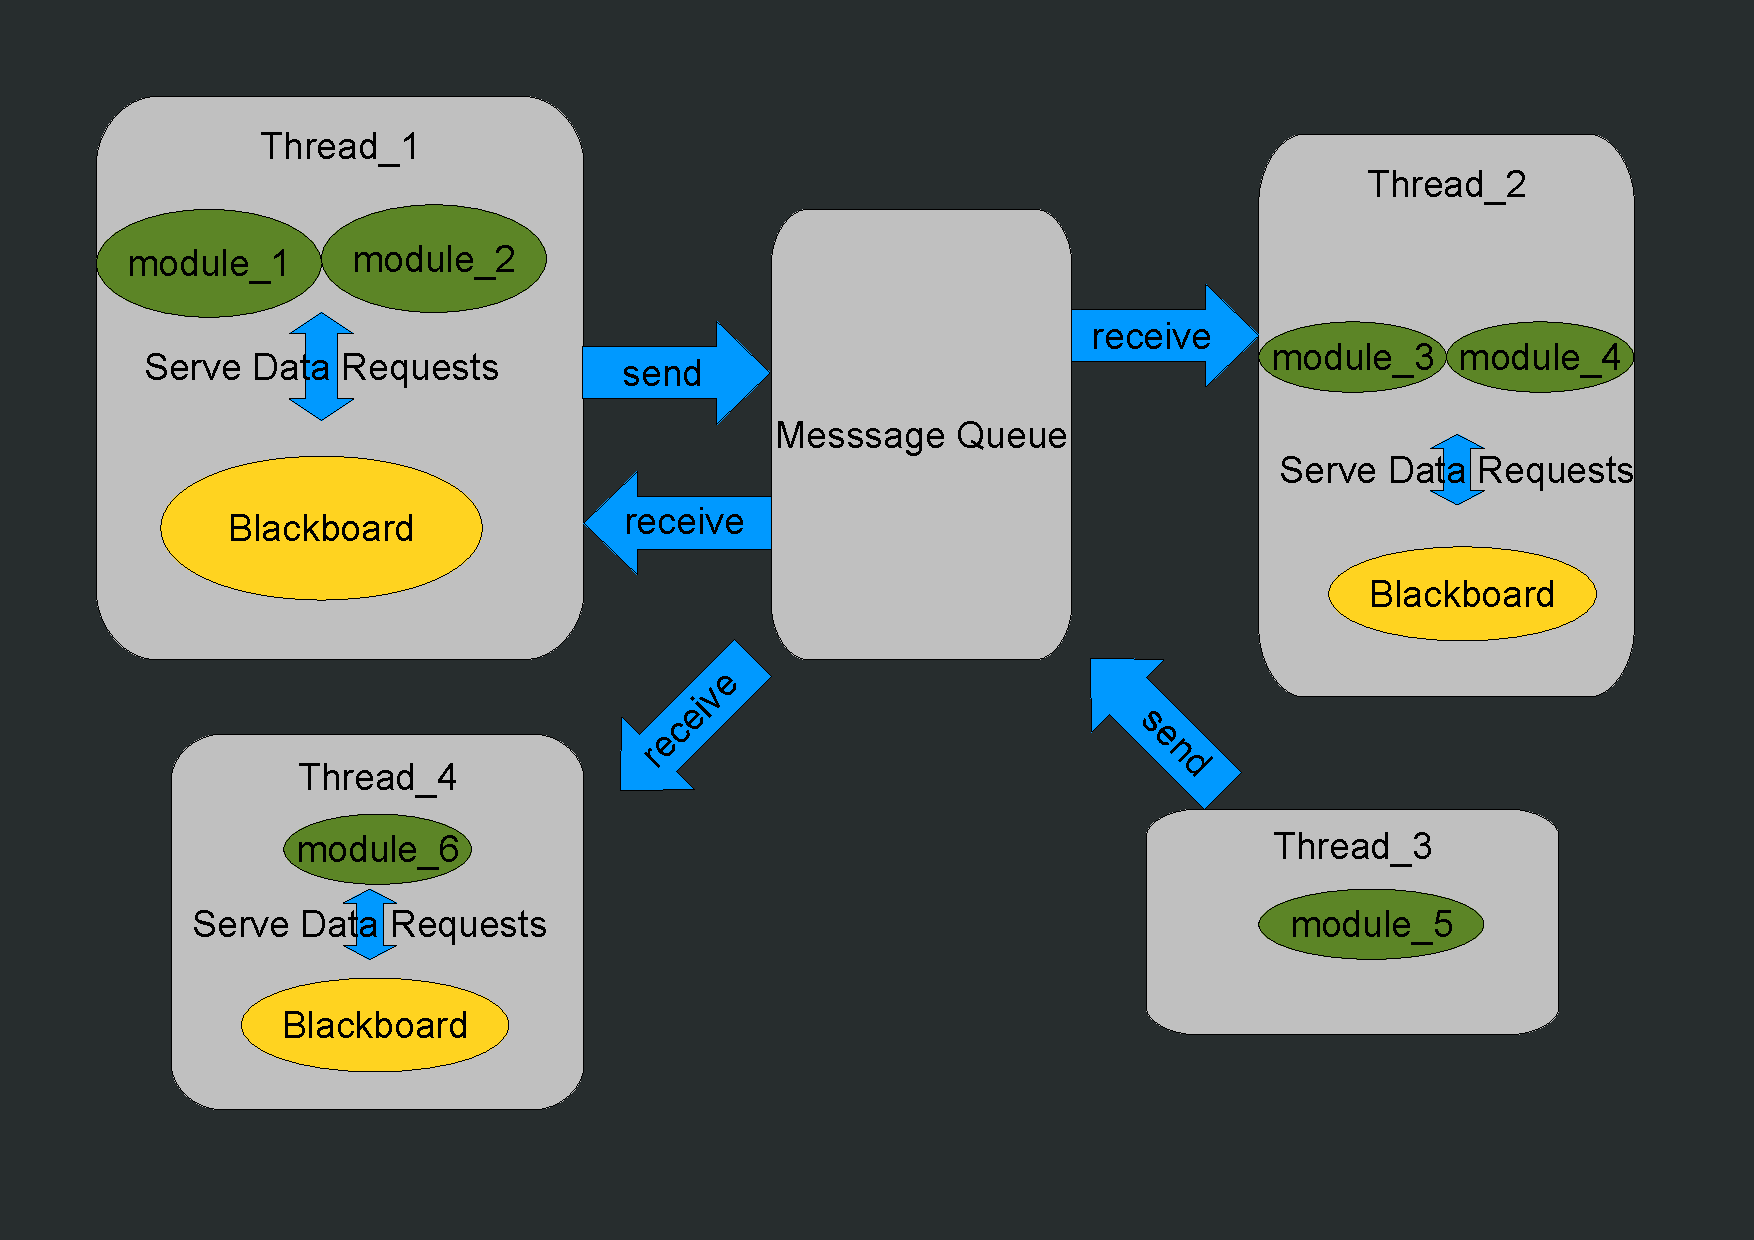
\includegraphics[width=0.6\columnwidth]{Chapter3/figures/new_architecture.pdf}
  \caption{Narukom's architecture.} 
  \label{fig:Narukom-architecture}
\end{figure}


\section{Data Serialization}
Serialization is a well-known issue when exchanging data over the network between heterogeneous systems. This issue was
a major concern when designing Narukom, consequentrly several frameworks  were assessed according four criteria
\begin{itemize}
\item { \tt Language support}, Support for both\textit{C++} and python  was a hard constraint as these two languages now used in the Nao platform,
\item User friendliness, users should have the ability to describe easy and quickly new data structures,
\item Cross-platform, \textit{Narukom} aimed to be a cross-platform framework and
\item Efficiency, the selected framework must be robust.
\end{itemize}
There were five main candidate solutions that were extensively reviewed , XML, CORBA, boost serialization library, google protocol buffers and a custom serialization method. Here, follows a brief comparison between those alternatives in order to make clear why we chose google protocol buffers over the other frameworks. XML met all our needs but efficiency, as extensive parsing of XML files is a resource draining procedure on a real-time system such as a robotic system. Although CORBA does meet all the criteria, it is not the ideal solution in terms of efficiency. Continuing  to boost library, failed in the terms of user friendliness requiring users to write their own serialization methods and at the same time there was no simple way to define new messages. The procedure is not painful, but it was preferred to follow a solution , which messages could be declared and described independent of a specific programming language. The development of our own serialization method, as tempting as it sounds, it would introduce serious debugging, code maintenance problems  not to mention that optimizing the whole procedure  is a long , painful path to follow. Finally, as far as protocol buffers are concered cover all our needs. Definition of messages is simple and intuitive , {\tt C++},{\tt python} are officially supported by Google and last but not least the code is heavily tested and optimized, all these made protocol buffers the ideal tool for constructing our hierarchical message structures.
Every message definition in Narukom takes the following form with five mandatory attributes in its preamble: 
\begin{verbatim}
message xxxMessage{
    required string host      = 1 [default = "localhost"];
    required string publisher = 2 [default = "" ];
    required string topic     = 3 [default = "global"];
    required int32  timeout   = 4 [default = 0];
    required string  timestamp = 5 [default = ""];
    < attributes specific to the xxxMessage type >
}
\end{verbatim} 
These five attributes can be characterized as the metadata of every message required by Narukom in order to provide its
services accurately. A short explanation of each of these attributes follows:
\begin{itemize}
\item {\tt host} is the unique name of the node sending the message
\item{\tt publisher} is the name of the publisher that generated the message
\item{\tt topic} is the topic to which the message belongs
\item{\tt timeout} is a 32-bit integer indicating the amount of time (in milliseconds) after which the message expires
and should be discarded from the Blackboard
\item{\tt timestamp} is a string indicating the absolute time at which the message was published and is used for
synchronization purposes between publishers and subscribers.
\end{itemize}



\section{Synchronization}

Synchronization among the modules of a robot is vital for accurate operation\footnote[2]{Anecdotal evidence for this claim includes our team's performance at RoboCup 2009, where the camera images processed by our vision module were not in synch with the robot head pose recorded by the behavior module, thus yielding erroneous object perceptions with catastrophic consequences on the robot's behavior.}. Narukom, in order to address the decoupling between publishers and subscribers, adds some synchronization information in the meta-data of each message ({\tt timeout} and {\tt timestamp}). Under this convention, the Blackboard's original interface had to be slightly altered to provide modules with synchronized data, should the need arises. If a module queries the Blackboard with a certain time stamp value, the Blackboard will have to find and return the data with the closest {\tt timestamp} value in the Blackboard. The {\tt timestamp} attribute is the absolute time at which the message was published to the Message Queue and the {\tt timeout} attribute is the (relative) amount of time (in milliseconds) indicating how long a subscriber should keep the message in its own Blackboard, counting from the time of arrival. The timeout mechanism is necessary for avoiding excess amounts of expired, useless data on the Blackboard. It should be stretched that these synchronization rules cannot be imposed and every subscriber has the flexibility to comply or not with those rules. Narukom's distributed
Blackboard implementation utilizes these two attributes in each message to achieve a balance between the length of the
synchronization period and the amount of memory needed for this purpose, allowing different settings for each message type.


\section{Communication within and across nodes}

Communication between threads running on the same node is implemented simply through the Message Queue of the node, as described already above. Communication between different nodes adopts a somewhat different approach. Given the publish/subscribe nature of Narukom, it is clear that the only missing part for communication over the network is a module, which subscribes to all topics and broadcasts over the network messages destined for other nodes, and at the
same time listens to broadcast traffic on the network and publishes the relevant messages on the local Message Queue. To this end, Narukom introduces the Catalog module. This module maintains contact information about the other nodes on the network and the type of data other nodes might be interested in. The first question we should address is why it is important to have this functionality. In a distributed system, especially in robotic environment, agents must be aware of all the on-line team members in order to utilize all the available resources for exchanging data across nodes, thus complex behaviors and distributed algorithms are much easier to be implemented.

\subsection{Channels}

A multi-purpose robot, such as Nao, has multiple means of interacting with its environment, either sensors or actuators.  Sensors (camera, network adapter,
microphones, etc.) sense the robot's environment, whereas actuators (motors, network adapter, speakers, etc.) affect the robot's environment.  If the effect of a robot's actuator is observable by another robot's sensor, this pair of actuator/sensor offers a possible communication channel. Narukom tries to integrate different channels into the framework. To do that introduces the catalog modules, which is responsible for holding contact information about any available peer in through Narukom's framework, at the same time is responsible for controlling the channels already implemented in Narukom.
 
 By default, the Catalog module establishes two channels: one listening for network-broadcast data from other peers and
another one for broadcasting data to all the reachable peers through network. Both channels use the UDP transmission
protocol. The Catalog Module establishes an extra incoming channel for interacting specifically with the game
controller, wherever there is such a need.
% Blackboard pro
% ------------------------------------------------------------------------

%%% Local Variables:
%%% mode: latex
%%% TeX-master: "../thesis"
%%% End:vides a simple interface with two methods the in and read. \tt{Read} returns the requested data , on the other hand \tt{in} first remove the data and then returns them to the module. The requests for data have the following form robot[x].publisher.type_of_message. Blackboard's transparent interface enables the user to access 